% CS329 final report, Group 11.  Compile: pdflatex main && bibtex-free (references inline) && pdflatex main
% Every table and figure below is generated by  experiments/make_report_assets.py  from the CSVs in results/.
\documentclass[10pt]{article}
\usepackage[a4paper,margin=0.9in]{geometry}
\usepackage[T1]{fontenc}
\usepackage{times}
\usepackage{amsmath,amssymb,amsthm}
\usepackage{booktabs,graphicx,xcolor}
\usepackage[hidelinks]{hyperref}
\usepackage{fancyhdr}
\usepackage{algorithm}
\usepackage{algpseudocode}
\usepackage{caption}
\usepackage{enumitem}
\usepackage[section]{placeins}
\captionsetup{font=small,labelfont=bf}
\setlist{nosep,leftmargin=1.2em}
\setlength{\parskip}{2pt}

% >>> replace with the public repository URL before submitting <<<
\newcommand{\repourl}{\url{https://github.com/<your-username>/strategic-deadlock}}

\pagestyle{fancy}
\fancyhf{}
\fancyhead[L]{\small Strategic Resource Contention and Deadlock in Multi-Agent Systems}
\fancyhead[R]{\small CS329 Final Report}
\fancyfoot[C]{\thepage}
\renewcommand{\headrulewidth}{0.4pt}

\newtheorem{definition}{Definition}
\newcommand{\PoAhat}{\widehat{\mathrm{PoA}}}
\newcommand{\Req}{\textsf{Request}}
\newcommand{\Hold}{\textsf{Hold}}
\newcommand{\Yield}{\textsf{Yield}}

\title{\vspace{-1.2em}\textbf{Strategic Resource Contention and Deadlock\\ in Multi-Agent Systems}}
\author{
\begin{tabular}{cccc}
Nityanand Karmali & Patil Nachiket Kiran & Devashish & Devvrat Hans\\
\small 24110226 & \small 24110250 & \small 24110104 & \small 23110094\\
\multicolumn{4}{c}{\small IIT Gandhinagar \quad\textbullet\quad Code: \repourl}
\end{tabular}}
\date{\vspace{-2em}}

\begin{document}
\maketitle

\begin{abstract}
\noindent Deadlock is classically an engineering bug that a central coordinator prevents, avoids or detects
(Banker's Algorithm, resource ordering, Wait-For-Graph detection)~\cite{dijkstra,coffman,havender}. We remove the
coordinator: each agent decides selfishly whether to \Req, \Hold\ or \Yield\ the locks it needs, so deadlock becomes a
possible outcome of rational play. We model decentralized lock acquisition as a finite-horizon stochastic
game~\cite{shapley}, solve the two-agent game exactly, and study three agents with best-response dynamics, fictitious play
and independent/shared Q-learning over a grid of 14{,}040 runs. We find that (i) exact two-agent equilibria almost never
deadlock (deadlock probability $\delta\le0.08$) but are still inefficient (Price of Anarchy up to $2.6$), and learning
agents on the same game do worse than the equilibrium; (ii) with three
agents, deadlock is driven by the \emph{dynamics}, not the payoffs: best-response dynamics on the dense topology deadlocks
for every $R/K\ge1$ (threshold $\theta\approx0.75$, independent of $D$), while Q-learners avoid deadlock but stall
instead; (iii) partial information lowers $\delta$ for every method; and (iv) a coordinator-free escalating holding cost
reduces the two-agent PoA from $1.81$ to $1.35$, but closes at most $\approx15\%$ of the gap to the centralized optimum for
three learning agents.
\end{abstract}

\section{Introduction}
Microservices, database transactions, warehouse robots and teams of LLM agents~\cite{guo} often need exclusive access to
several shared resources at once. If a resource is busy an agent can keep what it has and wait, or give everything back.
Coffman et al.~\cite{coffman} showed that deadlock needs mutual exclusion, hold-and-wait, no preemption and a circular
wait, visible as a cycle in the Wait-For Graph. The classical remedies~\cite{dijkstra,havender} all assume an authority or
a universally obeyed convention. Without one, three agents in a ring (agent $i$ holds $R_i$ and needs $R_{i+1}$) face a war
of attrition~\cite{maynard}: whoever yields pays, the others benefit, so everyone prefers that someone else yields.
We therefore ask \emph{when} selfish agents settle into deadlock (RQ1) and whether an incentive that each agent computes
for itself, a holding cost that escalates with holding time, can move them away from it (RQ2). The loss is measured by the
Price of Anarchy (PoA)~\cite{kp,roughgarden} against a centralized optimum. Congestion games~\cite{rosenthal} have no
hold-and-wait and multi-agent RL~\cite{busoniu} has not studied lock contention; our model combines the two.
\textbf{This report} adds to the reviewed proposal the algorithms we implemented (Section~\ref{sec:method}), the results
(Section~\ref{sec:results}) and the contribution of each member (Section~\ref{sec:contrib}). All numbers are reproduced by
the code in the repository (Appendix~\ref{sec:repro}).

\section{Model}\label{sec:model}
\textbf{Game.} Agents $N=\{1,\dots,n\}$ share single-unit locks $\mathcal R=\{R_1,\dots,R_m\}$. Agent $i$ needs
$\mathcal R_i\subseteq\mathcal R$ in a fixed order $o_i$. The state is $s=(\sigma,(h_i,\kappa_i,d_i)_i)$: the allocation
$\sigma$, the holding time $h_i$, a cooldown $\kappa_i\in\{0,\dots,\tau_{\max}\}$ after a yield, and a completion flag
$d_i$. Agents with $d_i=1$ or $\kappa_i>0$ can only \Hold; otherwise $A_i=\{\Req,\Hold,\Yield\}$. All agents act
simultaneously and the transition applies, in order, (T1) release on \Yield\ with $\kappa_i\sim\mathrm{Unif}\{1..\tau_{\max}\}$,
(T2) grant each free resource to one uniformly random requester whose next lock it is, (T3) complete and release when
$\mathcal R_i$ is held, (T4) update $h_i,\kappa_i$. The Wait-For Graph $G_t$ has an edge $i\to j$ iff $i$ requested,
was not granted, and its next lock is held by $j$; $C(G_t)$ is the set of agents on a directed cycle.

\textbf{Payoff.} With the escalating holding cost $\varphi_\rho(h)=c_0(1+\rho)^h$,
\begin{equation}\label{eq:payoff}
u^\rho_i = R\,\mathbf 1[\text{$i$ completes}] - \varphi_\rho(h_i)\,\mathbf 1[\text{$i$ incomplete and holds a lock}]
 - K\,\mathbf 1[a_i=\Yield] - D\,\mathbf 1[i\in C(G_t)] .
\end{equation}
$\rho=0$ is the baseline game $\Gamma_0$; $\rho>0$ is the RQ2 mechanism, computed by each agent from its own $h_i$, so
no third party enforces it. Each agent maximizes its own discounted return ($\gamma=0.95$, horizon $H=20$).

\textbf{Observations.} Agent $i$ sees $o^{\text{full}}_i=(k_i,\min(h_i,\bar h),\mathbf 1[\kappa_i>0],\mathbf 1[i\in
C(G_{t-1})])$ or, under partial information, the last bit replaced by ``my next lock is taken''.

\textbf{Known and unknown.} The experimenter knows the game ($N$, $(\mathcal R_i,o_i)$, $R,K,D,c_0,\rho,\tau_{\max},H,L$).
Each agent does not know the others' policies $\pi_{-i}$ and, under partial information, the global Wait-For Graph. We
therefore compare methods that \emph{know} the model (exact SPE, best-response dynamics, $C^\star$, Banker's) with methods
that must \emph{learn} it from play (Q-learning), which is the full-information versus learning comparison of the
course project directions.

\textbf{Metrics.} A \emph{deadlock episode} has $C(G_t)\neq\emptyset$ for $L=4$ consecutive steps; a \emph{livelock
episode} is not a deadlock, ends with an incomplete agent, and has a \Yield\ in every window of $L$ steps. We add a third
failure mode found in the experiments: a \emph{stall episode} ends incomplete but is neither (agents wait without a circular
wait or yields). $\delta,\lambda$ are the probabilities of deadlock and livelock. The social cost
$C(\pi)=\sum_i(R-U^0_i(\pi))\ge0$ uses the undiscounted base payoff ($\rho=0$), $C^\star=\min_{\pi_c}C(\pi_c)$ is the
centralized optimum, $\PoAhat(\pi)=C(\pi)/C^\star$, and the PoA is the worst $\PoAhat$ over equilibria. The exploitability
$\varepsilon(\pi)=\max_i[\max_{\pi'_i}U_i(\pi'_i,\pi_{-i})-U_i(\pi)]$ checks equilibrium claims, and the fraction of the
gap closed by the mechanism is
\begin{equation}\label{eq:g}
g(\rho)=\frac{C(\pi^{eq}_0)-C(\pi^{eq}_\rho)}{C(\pi^{eq}_0)-C^\star}.
\end{equation}

\textbf{Research questions.} \emph{RQ1}: is $\delta$ a threshold function of $R/K$, i.e.\ is there a $\theta(n,T,I,D)$ at
which $\delta$ crosses $\tfrac12$, and how does it move with topology $T$ and information $I$? \emph{RQ2}: for $\rho>0$,
is $C(\pi^{eq}_\rho)<C(\pi^{eq}_0)$, and how large is $g(\rho)$?

\section{Methodology}\label{sec:method}
The implementation is a Python package (\texttt{deadlock\_game}) with one module per proposal stage. All solvers below
are \emph{exact} where the proposal allowed it; learning is used only where exact computation is intractable.

\textbf{Stage 0: simulator.} \texttt{DeadlockEnv.step(state, actions, rng)} implements T1--T4 and Eq.~\eqref{eq:payoff},
with Tarjan's strongly-connected-components algorithm for $C(G_t)$ and seeded randomness for tie-breaking and cooldowns.
Holdings are always a prefix of $o_i$, so $\sigma$ is stored as the number of locks held, and for $\rho=0$, $h_i$ is capped
at $\bar h=4$ (it only matters through the observation). This makes the joint state space small enough for exact
methods: besides sampling, \texttt{env.transitions(s,a)} enumerates every successor with its exact probability.
23 unit tests cover the transition rules, hand-checked ring traces, cycle detection, the metric definitions and the solvers.

\textbf{Exact policy evaluation, best response, $\varepsilon$ and $C^\star$.} For a fixed (possibly randomized) profile
we propagate the state-occupancy distribution forward over $t=0..H$ to get every agent's exact return. A best response of
agent $i$ is computed by backward induction over $(t,s)$ on the single-agent MDP induced by $\pi_{-i}$. Because the
deviator sees the full state and time, the resulting $\varepsilon$ is an \emph{upper bound} on exploitability within
observation-based policies, the conservative direction for equilibrium claims. $C^\star$ is a dynamic program over
\emph{joint} actions ($3^n$ per state) with the base payoff. Monte-Carlo estimates agree with the exact values (unit test).

\begin{algorithm}[t]
\caption{Stage 1: subgame-perfect equilibrium of the two-agent game by backward induction}\label{alg:spe}
\small
\begin{algorithmic}[1]
\State $V_k(H,s)\gets0$ for all $s$, $k\in\{1,2\}$
\For{$t=H-1,\dots,0$} \textbf{for} every state $s$ reachable at time $t$
  \State $M_k[a_1,a_2]\gets\sum_{s'}P(s'\mid s,a)\,\bigl(u^\rho_k(s,a,s')+\gamma V_k(t{+}1,s')\bigr)$ \Comment{$M_\rho(h)$ + continuation}
  \State $\mathcal E\gets$ all Nash equilibria of $(M_1,M_2)$ (nashpy~\cite{knight} support enumeration $\cup$ pure-NE check)
  \State $(x,y)\gets$ \textsc{Select}$(\mathcal E)$ \Comment{symmetric (default), welfare-max, or welfare-min}
  \State $V_k(t,s)\gets x^\top M_k y$; \ store $\pi_t(s)=(x,y)$
\EndFor
\State $h^\star\gets$ first holding time at which $\Yield$ is in the on-path support; evaluate $\delta,\lambda,C,\PoAhat,\varepsilon$
\end{algorithmic}
\end{algorithm}

\textbf{Stage 1: exact two-agent equilibria} (Algorithm~\ref{alg:spe}). For the standoff topology
($o_1=(R_1,R_2)$, $o_2=(R_2,R_1)$) we solve the \emph{whole} finite game, not only the one-shot matrix: at each $(t,s)$ the
stage game is $M_\rho(h)$ of the proposal plus continuation values. The selection rule matters because the game is
symmetric and agents cannot coordinate who yields; we report the symmetric selection and use welfare-max/welfare-min to
bound the PoA. Each SPE's exploitability is computed independently as a check.

\begin{algorithm}[t]
\caption{Stage 2: best-response dynamics with observation projection}\label{alg:brd}
\small
\begin{algorithmic}[1]
\State $\pi^{(0)}\gets$ always-\Req; \ $\mathcal S\gets\{\mathrm{sig}(\pi^{(0)})\}$
\For{$r=1,\dots,20$}
  \For{each agent $i$ (simultaneously)}
    \State $Q_i(t,s,\cdot)\gets$ exact best response to $\pi^{(r-1)}_{-i}$ (backward induction)
    \State $\pi^{(r)}_i(o)\gets\arg\max_a\sum_{(t,s):\,o_i(s)=o}\mu^{(r-1)}(t,s)\,Q_i(t,s,a)$ \Comment{occupancy-weighted projection}
  \EndFor
  \State \textbf{if} $\mathrm{sig}(\pi^{(r)})=\mathrm{sig}(\pi^{(r-1)})$ \textbf{then} converged; \textbf{else if} $\mathrm{sig}(\pi^{(r)})\in\mathcal S$ \textbf{then} cycle detected; stop
  \State $\mathcal S\gets\mathcal S\cup\{\mathrm{sig}(\pi^{(r)})\}$
\EndFor
\State \Return $\pi^{(r)}$, converged/cycled flag, $\varepsilon(\pi^{(r)})$
\end{algorithmic}
\end{algorithm}

\textbf{Stage 2: best-response dynamics} (Algorithm~\ref{alg:brd}) for $n=m=3$ on the \emph{ring}
($\mathcal R_i=\{R_i,R_{i+1}\}$) and \emph{dense} (every agent needs all three locks, random orders redrawn until a circular
wait is reachable) topologies. Agents can only condition on observations, so the full-state best response is projected
onto observation policies with the occupancy-weighted $Q$-value. We stop at a fixed point, at a revisited profile (a cycle),
or after 20 rounds.

\textbf{Stage 3: learned policies.} (a) \emph{Independent Q-learning}~\cite{watkins}: one table per agent, $\alpha=0.1$,
$\epsilon$-greedy exploration decaying linearly from $1$ to $0.05$ over 2000 episodes. (b) \emph{Parameter-shared
Q-learning}: one table updated with every agent's experience, each agent acting on its own $o_i$, with decaying step
$\alpha_e=0.1/(1+e/1000)$ against non-stationarity~\cite{tan,claus}. Both stop after 5000 episodes or when the greedy
policy is unchanged for 200 episodes (after at least 500). (c) \emph{Fictitious play}~\cite{brown}: each iteration every
agent plays an exact (projected) best response to the others' \emph{average} policy; averages are updated with step
$1/(k{+}1)$ for 15 iterations. Every learned profile is evaluated on 500 Monte-Carlo episodes and its $\varepsilon$ is
computed exactly.

\textbf{Stage 4 and baselines.} Stage 3 is re-run for $\rho\in\{0.05,0.1,0.2,0.5\}$. The baselines are
\emph{always-\Req}; \emph{Banker's Algorithm}~\cite{dijkstra} (centralized, knows every $\mathcal R_i$, grants a request
only if the resulting state is safe, at most one grant per lock per step); \emph{resource ordering}~\cite{havender} (all
$o_i$ follow one global order); \emph{randomized exponential back-off}~\cite{metcalfe} (yield after $w=2$ failed requests,
then wait $\mathrm{Unif}\{1..2^{\min(j,4)}\}$ steps); and the centralized optimum $C^\star$.

\textbf{Grid and statistics.} $R/K\in\{0.5,1,2,4,8\}$ ($K=4$, $c_0=1$), $D/c_0\in\{0,0.1,0.56,3.16,17.8,100\}$,
$\rho\in\{0,.05,.1,.2,.5\}$, $I\in\{\text{full},\text{part}\}$, two topologies, 10 seeds for every stochastic method
(Q-learning, back-off): 14{,}040 runs, $\approx29$ CPU-hours. Deterministic solvers (BRD, FP, SPE, Banker's, ordering,
$C^\star$) are run once per cell. To compare with Stage 1, every method is also run on the two-agent standoff over the
same grid (7{,}320 further runs). We report means with 95\% Student-$t$ intervals, and test RQ2 per cell with a paired
$t$-test over seeds ($p<0.05$).

\section{Results}\label{sec:results}

\subsection{Stage 1: two agents almost never deadlock, but are inefficient}
\begin{figure}[t]
\centering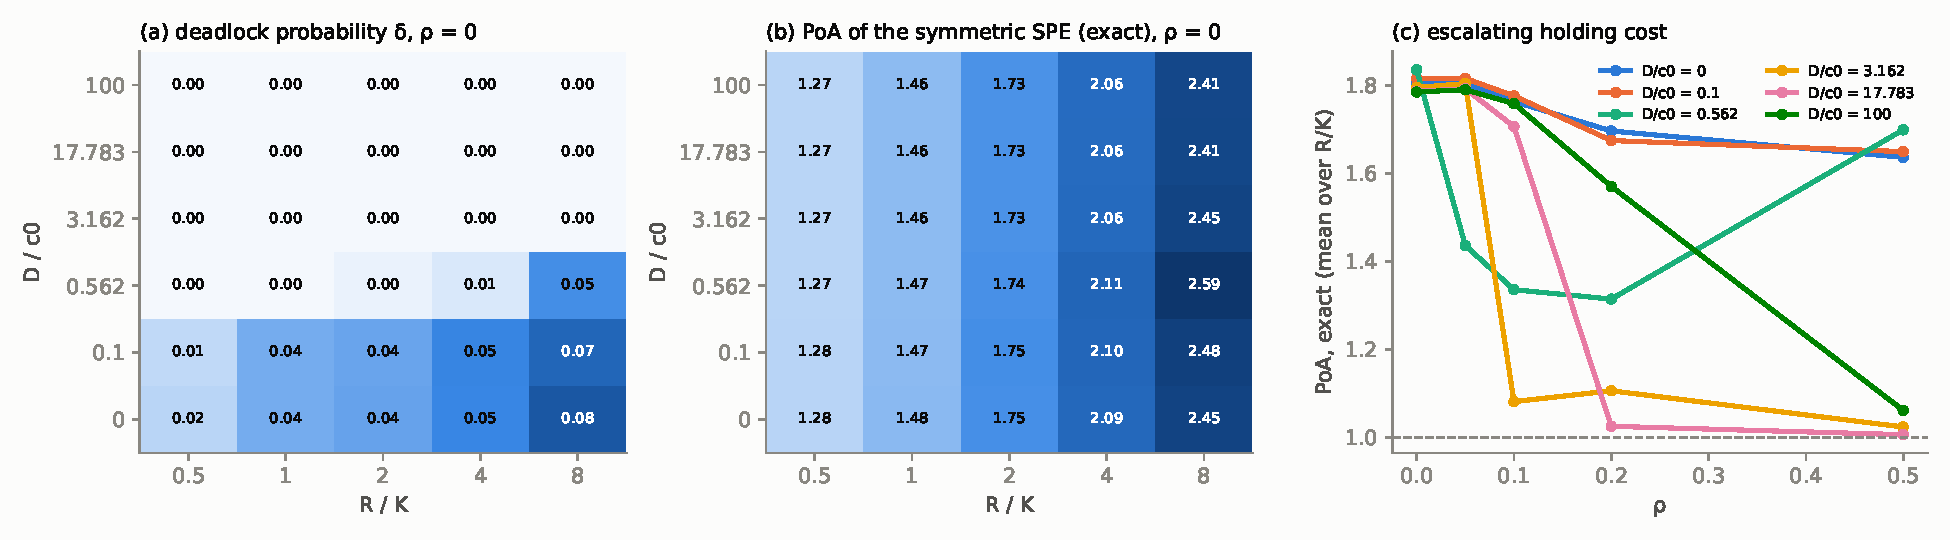
\includegraphics[width=\linewidth]{figures/fig_stage1.pdf}
\caption{Exact two-agent SPE (standoff topology). (a) $\delta$ is at most $0.08$ and vanishes for $D/c_0\ge3.16$.
(b) The exact $C/C^\star$ grows with $R/K$ and hardly depends on $D$. (c) The escalating holding cost lowers it for
every $D$; for $D/c_0\ge3.16$ it comes within 6\% of the optimum at $\rho=0.5$.}
\label{fig:stage1}
\end{figure}
\begin{table}[t]
\centering\small
\caption{Stage 1 by $R/K$ (each row aggregates the six $D$ values, $\rho=0$ unless stated). PoA band: best and worst
equilibrium selection. Costs are computed exactly (forward evaluation of the SPE), $\delta$ by 1000 simulated episodes.
$\varepsilon$: exploitability of the computed SPE.}
\label{tab:stage1}
\begin{tabular}{rrrrcrr}
\toprule
$R/K$ & $h^\star$ & $\max_D \delta$ & $C/C^\star$ & PoA band & $C/C^\star$ at $\rho{=}0.5$ & $\varepsilon$ \\
\midrule
0.5 & 1 & 0.02 & 1.27 & [1.00, 1.28] & 1.12 & $<10^{-9}$ \\
1 & 1 & 0.04 & 1.47 & [1.00, 1.48] & 1.20 & $<10^{-9}$ \\
2 & 1 & 0.04 & 1.74 & [1.00, 1.75] & 1.29 & $<10^{-9}$ \\
4 & 1 & 0.05 & 2.08 & [1.00, 2.11] & 1.46 & $<10^{-9}$ \\
8 & 1 & 0.08 & 2.46 & [1.00, 2.59] & 1.66 & $<10^{-9}$ \\
\bottomrule
\end{tabular}

\end{table}

Figure~\ref{fig:stage1} and Table~\ref{tab:stage1} show the exact two-agent results. Yield enters the equilibrium support
at the first holding step ($h^\star=1$) in every cell: when both agents hold their first lock, the symmetric equilibrium
mixes between \Req\ and \Yield\ immediately, as in a war of attrition. Deadlock therefore stays rare ($\delta\le0.08$),
occurs only when the circular-wait penalty is small ($D/c_0\le0.56$), and $\delta$ never crosses $\tfrac12$, so the
two-agent game has \emph{no} threshold $\theta$. The cost of selfishness shows up elsewhere: the symmetric equilibrium
wastes time in mixed standoffs, so $C/C^\star$ rises from $1.27$ at $R/K=0.5$ to $2.46$ at $R/K=8$ (the bigger the prize, the
longer both insist), and depending on which equilibrium is selected the PoA ranges from $1.0$ to $2.6$. The computed SPEs
have $\varepsilon<10^{-12}$, confirming they are equilibria.

\textbf{RQ2 for two agents.} The escalating holding cost works: averaged over the grid, $C/C^\star$ falls from $1.81$
($\rho=0$) to $1.74,\,1.57,\,1.40,\,1.35$ for $\rho=0.05,0.1,0.2,0.5$. For $D/c_0=17.8$ it reaches $1.03$ already at
$\rho=0.2$ ($g\approx0.96$). The effect is not monotone everywhere: for $D/c_0=0.56$, $C/C^\star$ drops to $1.31$ at
$\rho=0.2$ and rises again to $1.70$ at $\rho=0.5$, presumably because a steep holding cost also charges the agent that wins the standoff while it
completes.

\subsection{Do the simulation methods reproduce the exact equilibrium?}
\begin{table}[t]
\centering\small
\caption{All methods on the two-agent standoff, the game solved exactly in Stage 1 ($\rho=0$, averaged over $R/K$,
$D$, $I$; Monte-Carlo estimates). $g(0.5)$: gap closed by the escalating holding cost at $\rho=0.5$.}
\label{tab:standoff}
\begin{tabular}{lrrrrrr}
\toprule
Profile ($n=2$) & $\delta$ & stall & compl. & $\widehat{\mathrm{PoA}}$ & med.\ $\varepsilon$ & $g(0.5)$ \\
\midrule
SPE & 0.02 & 0.01 & 0.99 & 1.79 & 0.00 & 0.56 \\
Best-response dyn. & 0.00 & 1.00 & 0.00 & 12.40 & 6.60 & 0.00 \\
Fictitious play & 0.11 & 0.16 & 0.82 & 29.69 & 2.92 & -0.17 \\
Independent Q & 0.00 & 0.41 & 0.78 & 3.55 & 5.62 & -0.03 \\
Shared Q & 0.02 & 0.65 & 0.33 & 11.00 & 7.78 & 0.01 \\
Exp. back-off & 0.00 & 0.15 & 0.89 & 74.11 & -- & -- \\
Banker's & 0.00 & 0.00 & 1.00 & 1.00 & -- & -- \\
Centralized ($C^\star$) & 0.00 & 0.00 & 1.00 & 1.00 & -- & -- \\
\bottomrule
\end{tabular}

\end{table}
To test success criterion~1 we ran Stages 2--3 on the same two-agent game (Table~\ref{tab:standoff}). None of them
reaches the exact equilibrium. Independent Q-learning comes closest ($\PoAhat=3.6$ against $1.8$ for the SPE) but
stalls in $41\%$ of episodes; shared Q stalls in $65\%$; best-response dynamics oscillates between both agents requesting
and both abstaining and ends in a permanent stall, as on the ring; fictitious play is the only method that deadlocks more
than the SPE ($\delta=0.11$). All learned profiles remain exploitable (median $\varepsilon$ $3$--$8$, against $0$ for
the SPE). The escalating holding cost also does not transfer: it closes $56\%$ of the gap for the SPE but
$g(0.5)\in[-0.17,0.01]$ for the learners. So the exact two-agent analysis is a lower bound on the inefficiency of selfish
play that adaptive agents do not reach; the extra loss comes from how they learn, not from the game itself.

\subsection{Three agents (RQ1): deadlock is driven by the dynamics}
\begin{figure}[t]
\centering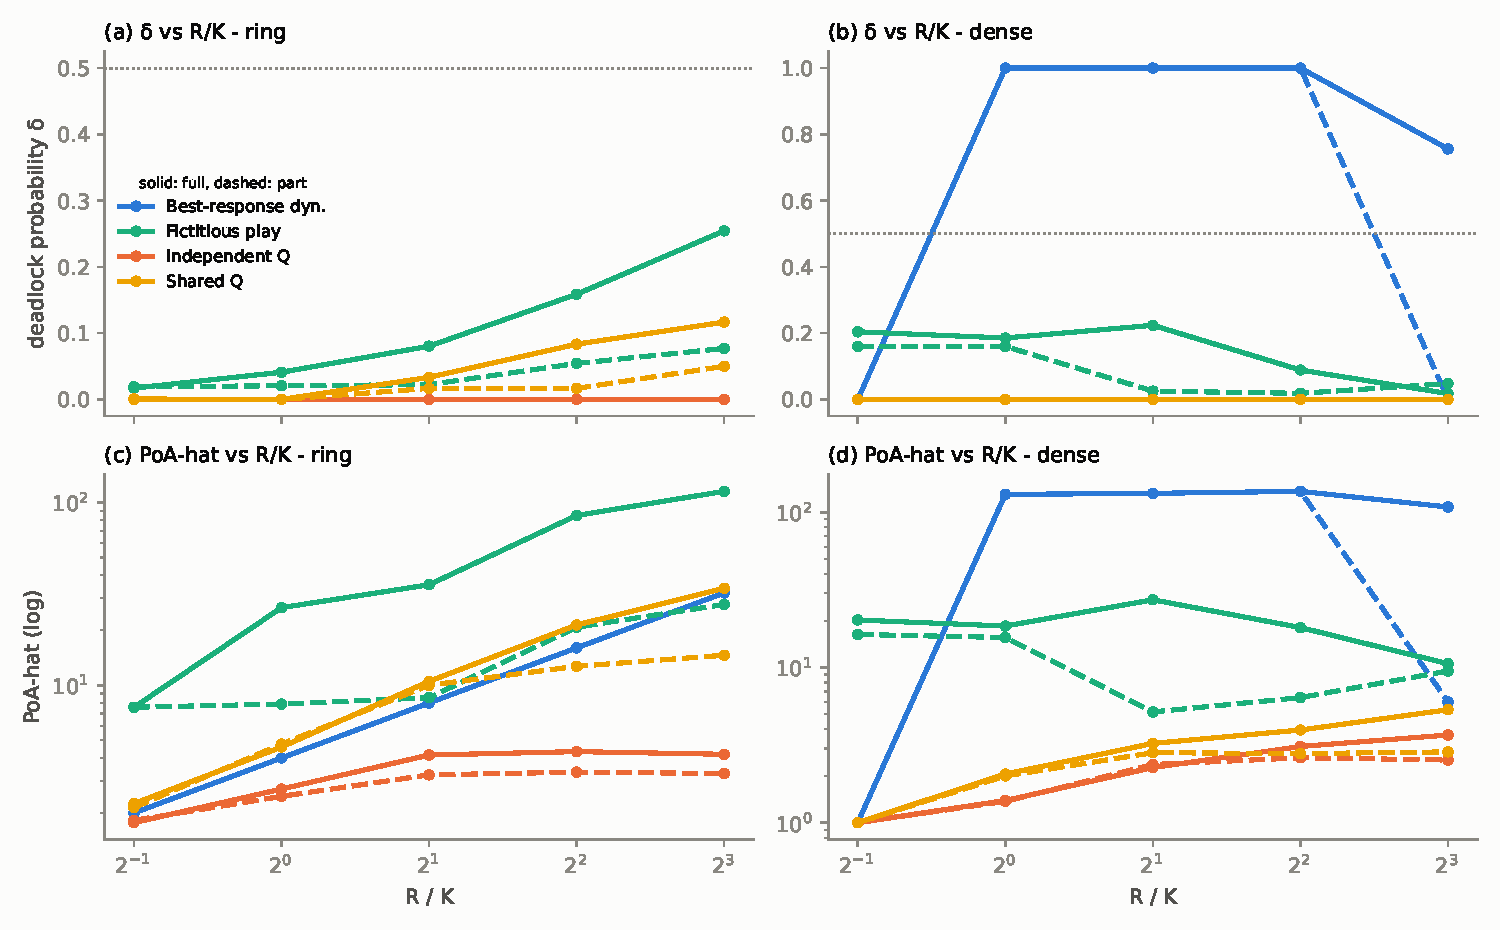
\includegraphics[width=0.9\linewidth]{figures/fig_rq1.pdf}
\caption{RQ1 at $\rho=0$, averaged over $D$. Top: deadlock probability; the dotted line is $\delta=\tfrac12$. Bottom:
$\PoAhat$ (log scale). Solid lines: full information, dashed: partial.}
\label{fig:rq1}
\end{figure}
\textbf{Deadlock threshold.} Only best-response dynamics on the dense topology produces a deadlock-dominated regime
(Figures~\ref{fig:rq1}b and~\ref{fig:regimes}): $\delta=0$ at $R/K=0.5$ and $\delta=1$ for $R/K\in\{1,2,4\}$, so
$\theta\approx0.75$ (linear interpolation), for \emph{every} $D$ and both information regimes. When completion is
worth little ($R/K=0.5$) best responses stop requesting; once it is worth more than a yield, each agent's best response to
the others' current policy is to insist, and with simultaneous updates all agents insist together. At $R/K=8$ the
dynamics sometimes escape ($\delta=0.76$ full, $0.04$ partial). This transition is a property of the \emph{dynamics}: BRD
converged in only 24\% (full) and 40\% (partial) of dense cells and cycled otherwise, and the reached profiles are far from
equilibrium (median $\varepsilon=22$). The penalty $D$ does not move $\theta$: by the time agents are in a cycle they are
already committed.

\begin{figure}[t]
\centering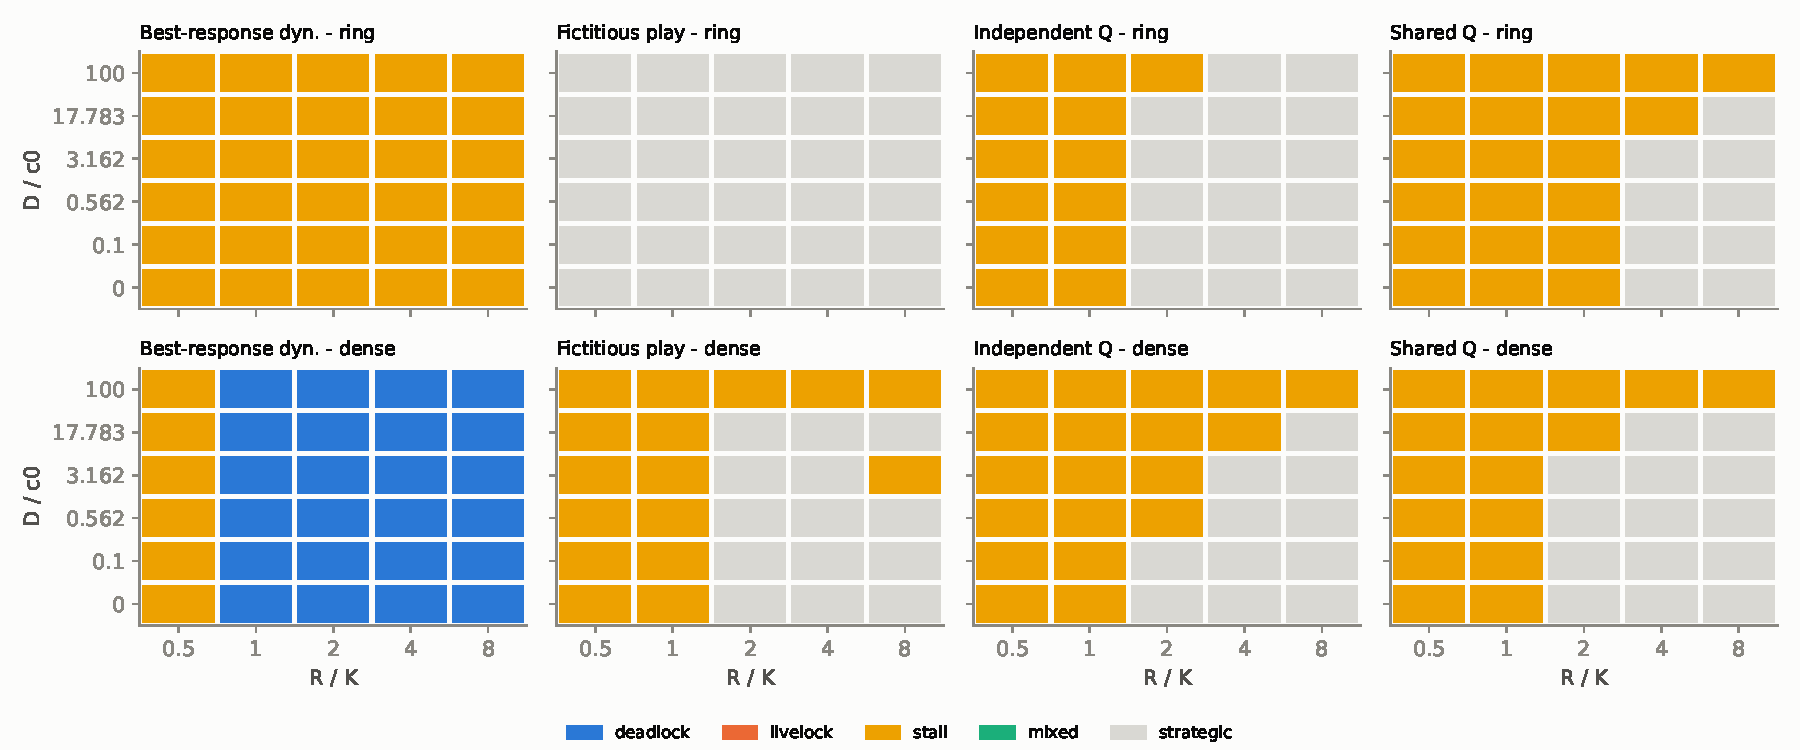
\includegraphics[width=0.92\linewidth]{figures/fig_regimes.pdf}
\caption{RQ1 regime map ($\rho=0$, full information): the outcome that dominates each $(R/K,D)$ cell. Deadlock/stall:
that outcome occurs in at least half of the episodes; strategic: deadlock, livelock and stall all below $\tfrac12$.
No cell is livelock-dominated or mixed.}
\label{fig:regimes}
\end{figure}

\textbf{Regime boundaries along $D$.} Figure~\ref{fig:regimes} answers the second part of RQ1. Only dense BRD has a
deadlock-dominated region; the alternative to strategic play is a \emph{stall}-dominated region at low $R/K$. For the
Q-learners the stall/strategic boundary moves to \emph{higher} $R/K$ as $D$ grows (e.g.\ independent Q on dense: strategic
from $R/K=2$ at $D\le0.1$, but only from $R/K=8$ at $D/c_0=17.8$, and never at $D/c_0=100$): a large circular-wait penalty
makes participating less attractive.

\textbf{Learners avoid deadlock.} Independent Q-learning never deadlocks, shared Q-learning has $\delta\le0.05$ on
average (at most $0.3$ in a single cell, $0$ on dense), and fictitious play stays below $0.35$ in every cell. On the ring, $\delta$ of FP and shared-Q \emph{rises} with
$R/K$ (from $0.02$ to $0.25$ for FP with full information), matching the intuition of RQ1, but never crosses
$\tfrac12$. Independent Q-learning is the most efficient selfish profile ($\PoAhat=3.1$ ring, $2.1$ dense) and the least
exploitable (median $\varepsilon\approx3$--$6$, against rewards of $2$--$32$); 70\% of its runs met the convergence rule,
against 52\% for shared Q. Contrary to our expectation, sharing parameters made learning \emph{less} stable: on the ring
the standard deviation of $C$ across the 10 seeds of a cell is $17.1$ for shared Q against $1.0$ for independent Q
(dense: $1.1$ vs $1.0$), visible as the wide confidence interval in Table~\ref{tab:methods}. With one table, all three
agents act on the same greedy policy, so symmetric standoffs cannot be broken by heterogeneous policies.

\textbf{Information.} Partial information lowers $\delta$ for every method that deadlocks (dense BRD $0.75\to0.60$,
dense FP $0.14\to0.08$, ring FP $0.11\to0.04$, ring shared-Q $0.047\to0.017$). One reading: an agent that only sees that its next lock is taken cannot tell a passing conflict from a circular wait,
and the learned policies respond to that uncertainty by waiting less aggressively.

\textbf{A third failure mode: stalls.} Livelock is essentially absent ($\lambda\le0.001$ on average), but many runs end
with incomplete agents anyway (Table~\ref{tab:methods}, Figure~\ref{fig:regimes}). On the ring, BRD \emph{always} cycles
with period two between ``everyone requests'' (deadlock) and ``nobody requests'' (each agent's best response to aggressive
opponents is to stay out); the profile at which the cycle is detected is the passive one, so no agent ever completes
($C=nR$, $\delta=\lambda=0$). Stalls end $39\%$ (independent Q) and $64\%$ (shared Q) of the
learners' ring episodes and about half of their dense episodes. Q-learners stall by \emph{abstaining}: in their incomplete episodes the unfinished agents hold no lock and never
request one. Abstention grows when completion is worth little (at $R/K=0.5$ abstaining is individually rational, since
the holding cost of three locks exceeds $R$) and when the circular-wait penalty is large: averaged over $R/K$, the
completion rate of shared Q on the ring falls from $0.34$ at $D=0$ to $0.19$ at $D/c_0=100$. A large $D$ does not cause
deadlock; it deters participation. The proposal's two-category taxonomy
(deadlock/livelock) therefore misses the most common failure of selfish agents in our model; we added the stall metric
to the code.

\begin{table}[t]
\centering\small
\caption{All profiles at $\rho=0$, averaged over $R/K$, $D$ and $I$. $\pm$: mean 95\% CI over seeds (stochastic
methods only). Latency: mean completion step of agents that finish. Seeds per cell; ``--'': not applicable (the
baselines are not equilibrium concepts).}
\label{tab:methods}
\begin{tabular}{lrrrrrrrr}
\toprule
Profile & seeds & $\delta$ & $\lambda$ & stall & compl. & latency & $\widehat{\mathrm{PoA}}$ ($\pm$95\% CI) & med.\ $\varepsilon$ \\
\midrule
\multicolumn{9}{l}{\emph{ring topology} ($C^\star=3$)} \\
Best-response dyn. & 1 & 0.00 & 0.00 & 1.00 & 0.00 & -- & 12.4 & 6.6 \\
Fictitious play & 1 & 0.07 & 0.00 & 0.07 & 0.90 & 5.9 & 34.2 & 3.4 \\
Independent Q & 10 & 0.00 & 0.00 & 0.39 & 0.82 & 3.6 & 3.1 $\pm$0.2 & 5.6 \\
Shared Q & 10 & 0.03 & 0.00 & 0.64 & 0.33 & 10.3 & 11.7 $\pm$4.1 & 8.3 \\
Always-request & 1 & 1.00 & 0.00 & 0.00 & 0.00 & -- & 417.5 & 48.5 \\
Exp. back-off & 10 & 0.00 & 0.00 & 0.06 & 0.97 & 11.7 & 59.2 $\pm$0.8 & -- \\
Banker's & 1 & 0.00 & 0.00 & 0.00 & 1.00 & 3.0 & 1.3 & -- \\
Resource ordering & 1 & 0.00 & 0.00 & 0.00 & 1.00 & 3.3 & 1.3 & -- \\
Centralized ($C^\star$) & 1 & 0.00 & 0.00 & 0.00 & 1.00 & 3.0 & 1.0 & -- \\
\midrule
\multicolumn{9}{l}{\emph{dense topology} ($C^\star=6$)} \\
Best-response dyn. & 1 & 0.68 & 0.00 & 0.30 & 0.09 & 5.2 & 91.4 & 22.3 \\
Fictitious play & 1 & 0.11 & 0.00 & 0.52 & 0.66 & 8.4 & 14.8 & 6.4 \\
Independent Q & 10 & 0.00 & 0.00 & 0.58 & 0.67 & 5.9 & 2.1 $\pm$0.1 & 2.8 \\
Shared Q & 10 & 0.00 & 0.00 & 0.46 & 0.54 & 7.4 & 2.7 $\pm$0.1 & 3.4 \\
Always-request & 1 & 1.00 & 0.00 & 0.00 & 0.00 & -- & 134.5 & 43.0 \\
Exp. back-off & 10 & 0.00 & 0.00 & 0.10 & 0.94 & 8.1 & 13.4 $\pm$0.2 & -- \\
Banker's & 1 & 0.00 & 0.00 & 0.00 & 1.00 & 6.0 & 1.0 & -- \\
Resource ordering & 1 & 0.00 & 0.00 & 0.00 & 1.00 & 6.0 & 1.0 & -- \\
Centralized ($C^\star$) & 1 & 0.00 & 0.00 & 0.00 & 1.00 & 6.0 & 1.0 & -- \\
\bottomrule
\end{tabular}

\end{table}

\subsection{Selfish profiles versus classical baselines}
Table~\ref{tab:methods} places the selfish profiles between the two classical extremes. Always-request deadlocks in
every episode ($\PoAhat=417$ ring, $134$ dense). Banker's Algorithm and resource ordering never deadlock and are optimal on
the dense topology ($C=C^\star=6$); on the ring they cost $4$ instead of $3$ ($\PoAhat=1.33$) because they serialize
agents that the optimum runs in parallel. Exponential back-off avoids deadlock too, but its blind waiting costs
$13$--$59\times C^\star$, worse than independent Q-learning ($2$--$3\times$). The same ordering holds for latency (mean completion step of
the agents that finish, Table~\ref{tab:methods}): independent Q finishes in $3.6$ (ring) and $5.9$ (dense) steps,
close to Banker's ($3.0$, $6.0$), while back-off needs $11.7$ and $8.1$. So the decentralized learners recover most of
what a coordinator buys, but not all of it.

\subsection{Stage 4 (RQ2): the escalating holding cost for three agents}
\begin{figure}[t]
\centering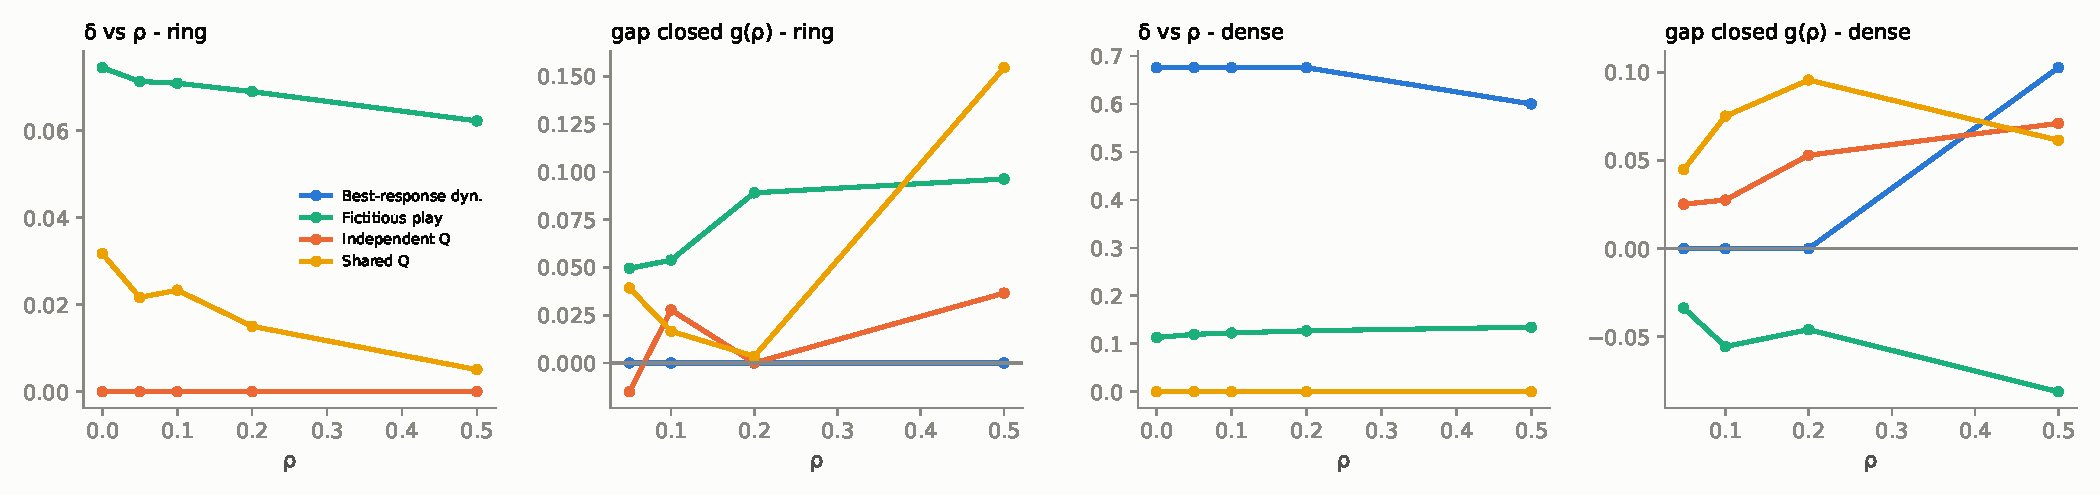
\includegraphics[width=\linewidth]{figures/fig_rq2.pdf}
\caption{RQ2: deadlock probability and gap closed $g(\rho)$ (Eq.~\ref{eq:g}) versus $\rho$, averaged over the grid.}
\label{fig:rq2}
\end{figure}
\begin{table}[t]
\centering\small
\caption{RQ2 for three agents. $g(\rho)$ averaged over $(R/K,D,I)$ cells; last column: number of the 60 cells in which
$C$ at $\rho=0.5$ is significantly lower/higher than at $\rho=0$ (paired $t$-test over 10 seeds, $p<0.05$; only for the
stochastic learners).}
\label{tab:rq2}
\begin{tabular}{llrrrrccc}
\toprule
Topology & Profile & $g(0.05)$ & $g(0.1)$ & $g(0.2)$ & $g(0.5)$ & $\delta$: $\rho{=}0\to0.5$ & $\widehat{\mathrm{PoA}}$: $\rho{=}0\to0.5$ & sig.\ $\downarrow/\uparrow$ \\
\midrule
ring & Best-response dyn. & 0.00 & 0.00 & 0.00 & 0.00 & 0.00$\to$0.00 & 12.4$\to$12.4 & -- \\
ring & Fictitious play & 0.05 & 0.05 & 0.09 & 0.10 & 0.07$\to$0.06 & 34.2$\to$31.3 & -- \\
ring & Independent Q & -0.02 & 0.03 & 0.00 & 0.04 & 0.00$\to$0.00 & 3.1$\to$3.0 & 5/0 \\
ring & Shared Q & 0.04 & 0.02 & 0.00 & 0.15 & 0.03$\to$0.01 & 11.7$\to$8.7 & 4/0 \\
dense & Best-response dyn. & 0.00 & 0.00 & 0.00 & 0.10 & 0.68$\to$0.60 & 91.4$\to$81.2 & -- \\
dense & Fictitious play & -0.03 & -0.06 & -0.05 & -0.08 & 0.11$\to$0.13 & 14.8$\to$16.0 & -- \\
dense & Independent Q & 0.03 & 0.03 & 0.05 & 0.07 & 0.00$\to$0.00 & 2.1$\to$2.1 & 15/1 \\
dense & Shared Q & 0.04 & 0.08 & 0.10 & 0.06 & 0.00$\to$0.00 & 2.7$\to$2.6 & 8/3 \\
\bottomrule
\end{tabular}

\end{table}
For three agents the mechanism helps, but modestly (Figure~\ref{fig:rq2}, Table~\ref{tab:rq2}). For Q-learners $C$
decreases on average for every $\rho\ge0.1$; at $\rho=0.5$ the decrease is statistically significant in 15 of 60 dense
cells for independent Q (1 significant increase) and in 4--8 cells for shared Q. Shared Q on the ring cuts $\delta$ from
$0.032$ to $0.005$ and $\PoAhat$ from $11.7$ to $8.7$ ($g=0.15$). Dense BRD escapes deadlock in some cells only at the
largest $\rho$ ($\delta$ $0.68\to0.60$, $g=0.10$), and fictitious play on the dense topology gets slightly \emph{worse}
($g<0$). We did not observe the feared trade of deadlock for livelock: $\lambda$ stays $\approx0$ for all $\rho$. The
difference to Stage 1 is that the three-agent losses come mostly from abstention stalls, which a holding cost (paid only
while holding) cannot fix: an agent that holds nothing pays nothing.

\subsection{Discussion against the success criteria}
\begin{enumerate}
\item \emph{Exact two-agent threshold reproduced in simulation:} partly. Stage 1 gives exact equilibria and $h^\star$, but
$\delta$ never reaches $\tfrac12$ for two agents, so there is no two-agent $\theta$. Run on the same game, the simulation
methods reproduce the low deadlock rate but not the equilibrium itself: they cost $2$--$16\times$ more and stall
(Table~\ref{tab:standoff}). A sharp threshold ($\theta\approx0.75$) appears only for three-agent best-response
dynamics.
\item \emph{Regions of reliable deadlock and livelock:} deadlock regions are clear: in the dense BRD cells with $R/K\in[1,4]$
$\delta=1.00$ in all 500 evaluation episodes, while independent Q has $\delta=0$ with a 95\% CI of $\pm0$ over 10 seeds,
so the intervals do not overlap; no livelock-dominated region exists; stalls take its place.
\item \emph{At least one $\rho>0$ reduces $C$ with a clear margin:} yes for two agents ($C/C^\star$ $1.81\to1.35$) and for
Q-learners in a minority of cells (paired tests above); $g(\rho)\le0.15$ on average for three agents.
\end{enumerate}
\textbf{Limitations.} $n=m=3$ is small because $C^\star$ and exact best responses need the joint state space. BRD and
FP are deterministic and run once per cell, so they have no confidence interval. The reported $\varepsilon$ is a full-state
upper bound. The compressed observations merge states, which partly explains the stalls.

\section{Contribution}\label{sec:contrib}
Each member owned one stage end to end and reviewed another, as planned in the proposal (Table~\ref{tab:contrib}).
\begin{table}[!htbp]
\centering\small
\caption{Task allocation from the proposal and its status. Paths refer to the repository.}
\label{tab:contrib}
\begin{tabular}{p{2.6cm}p{8.6cm}p{1.6cm}p{1.8cm}}
\toprule
Member & Assigned tasks (code) & Reviewed & Status\\
\midrule
Nityanand Karmali (24110226) & Game formulation; Stage 1 two-agent SPE via nashpy, $h^\star$, $\theta$
(\texttt{two\_agent.py}, \texttt{stage1\_two\_agent.py}); metrics, PoA, $g(\rho)$, CIs (\texttt{metrics.py});
plots and report (\texttt{make\_plots.py}, \texttt{make\_report\_assets.py}) & Stage 3 & Completed \\
Patil Nachiket Kiran (24110250) & Stage 0 simulator: \texttt{step()}, T1--T4, tie-breaking, cooldowns, Wait-For-Graph cycle
detection, logging (\texttt{env.py}, \texttt{wfg.py}); centralized optimum $C^\star$ and Banker's Algorithm
(\texttt{exact.py}, \texttt{baselines.py}); unit tests & Stage 1 & Completed \\
Devashish (24110104) & Stage 2 best-response dynamics (\texttt{best\_response.py}); exponential back-off and resource
ordering (\texttt{policies.py}, \texttt{baselines.py}); grid runner with seeds, checkpointing and CIs
(\texttt{experiments.py}, \texttt{run\_grid.py}) & Stage 0 & Completed \\
Devvrat Hans (23110094) & Stage 3 independent Q-learning, fictitious play, shared Q-learning, convergence rule,
exploitability (\texttt{learning.py}, \texttt{exact.py}); Stage 4 $\rho$ sweep and RQ2 analysis & Stage 2 & Completed \\
\bottomrule
\end{tabular}
\end{table}

\noindent The optional extensions named in the proposal (priority auctions, payments for preemption) were not attempted.
The stall metric was added beyond the plan after the Stage 2 results.

\section{Conclusion}
Without a coordinator, two selfish agents resolve standoffs almost immediately but inefficiently, and an escalating
holding cost removes most of that inefficiency. With three agents, whether they deadlock depends less on the payoffs than
on how they adapt: myopic simultaneous best responses lock the dense topology into deadlock for every $R/K\ge1$, while
Q-learners avoid deadlock but stall by abstaining, more so when the deadlock penalty is high. Less information makes agents more cautious and deadlock less likely. A
self-computed holding cost is safe (it never created livelock) but closes at most about 15\% of the gap to the optimum for
three learning agents, because it does not act on agents that hold nothing. Mechanisms that reward \emph{progress}, rather
than only taxing holding, are the natural next step.

\appendix
\section{Reproducibility}\label{sec:repro}
Repository: \repourl. Every figure and table in this report is written by \texttt{experiments/make\_report\_assets.py}
from the CSV files produced by the commands below; the numbers quoted in the text are printed to
\texttt{report/numbers.txt}. All randomness is seeded: the stall re-run of the 780 $\rho=0$ cells reproduced the social cost of the main run
in every cell (largest difference $10^{-13}$).
\begin{verbatim}
make setup && make test        # 23 unit tests
python experiments/stage1_two_agent.py --out results/stage1
python experiments/run_grid.py --preset all --out results/all   # 14,040 runs
make outcomes                  # rho = 0 cells with the stall metric
make standoff                  # all methods on the two-agent game
make report                    # tables, figures, numbers.txt, PDF
\end{verbatim}

\begin{thebibliography}{99}\small\setlength{\itemsep}{0pt}
\bibitem{dijkstra} E.~W. Dijkstra. Cooperating sequential processes. In \emph{Programming Languages}, Academic Press, 1968.
\bibitem{coffman} E.~G. Coffman, M.~J. Elphick, A.~Shoshani. System deadlocks. \emph{ACM Computing Surveys} 3(2), 1971.
\bibitem{havender} J.~W. Havender. Avoiding deadlock in multitasking systems. \emph{IBM Systems Journal} 7(2), 1968.
\bibitem{shapley} L.~S. Shapley. Stochastic games. \emph{PNAS} 39(10), 1953.
\bibitem{kp} E.~Koutsoupias, C.~H. Papadimitriou. Worst-case equilibria. \emph{STACS}, 1999.
\bibitem{roughgarden} T.~Roughgarden, \'E.~Tardos. How bad is selfish routing? \emph{JACM} 49(2), 2002.
\bibitem{metcalfe} R.~M. Metcalfe, D.~R. Boggs. Ethernet: distributed packet switching for local computer networks. \emph{CACM} 19(7), 1976.
\bibitem{guo} T.~Guo et al. Large language model based multi-agents: a survey of progress and challenges. \emph{IJCAI}, 2024.
\bibitem{maynard} J.~Maynard Smith. The theory of games and the evolution of animal conflicts. \emph{J. Theor. Biol.} 47(1), 1974.
\bibitem{rosenthal} R.~W. Rosenthal. A class of games possessing pure-strategy Nash equilibria. \emph{IJGT} 2(1), 1973.
\bibitem{busoniu} L.~Bu\c{s}oniu, R.~Babu\v{s}ka, B.~De~Schutter. A comprehensive survey of multiagent reinforcement learning. \emph{IEEE SMC-C} 38(2), 2008.
\bibitem{knight} V.~Knight, J.~Campbell. Nashpy: a Python library for the computation of Nash equilibria. \emph{JOSS} 3(30), 2018.
\bibitem{watkins} C.~J.~C.~H. Watkins, P.~Dayan. Q-learning. \emph{Machine Learning} 8(3--4), 1992.
\bibitem{brown} G.~W. Brown. Iterative solution of games by fictitious play. In \emph{Activity Analysis of Production and Allocation}, 1951.
\bibitem{tan} M.~Tan. Multi-agent reinforcement learning: independent vs.\ cooperative agents. \emph{ICML}, 1993.
\bibitem{claus} C.~Claus, C.~Boutilier. The dynamics of reinforcement learning in cooperative multiagent systems. \emph{AAAI}, 1998.
\end{thebibliography}
\end{document}
